\documentclass[a4paper]{article}

\usepackage{amsfonts, amsmath, amssymb, amsthm}
\usepackage{graphicx}
\usepackage{fullpage}
\usepackage{float}

\newtheorem{lemma}{Lemma}
\newtheorem{theorem}{Theorem}
\newtheorem{corollary}{Corollary}
\newtheorem{conjecture}{Conjecture}
\newtheorem{example}{Example}

\newcommand{\Z}{\mathbb{Z}}
\newcommand{\N}{\mathbb{N}}
\renewcommand{\qedsymbol}{$\blacksquare$}
\newcommand{\abs}[1]{\left| #1 \right|}
\renewcommand{\dim}[1]{\text{dim}\left( #1 \right)}
\newcommand{\xor}{\oplus}

\setlength{\parindent}{0em}
\setlength{\parskip}{1em}

\begin{document}
	\title{Resolution to Sutner's Conjecture}
	\author{William Boyles}
	\date{\today}
	\maketitle
	
	\section{Introduction}
	We resolve a conjecture first stated by Sutner in 1989 about the nullity of \textit{Lights Out} boards of size $2n + 1$ in the affirmative \cite{Sutner1989}.
	
	\section{Fibonacci Polynomials \& Rule 90}
	Let $d(n)$ be the nullity of an $n \times n$ \textit{Lights Out} board.
	Hunziker, Machiavelo, and Park showed \cite{HUNZIKER2004465}
	
	\begin{theorem}[Hunziker, Machiavelo, and Park]
		Let $f_n(x)$ be the degree $n$ polynomial in the ring $\Z_2[x]$ defined recursively by
		\begin{equation*}
			f_n(x) = \begin{cases}
				1 & n=0 \\
				x & n=1 \\
				xf_{n-1}(x) + f_{n-2}(x) & \text{otherwise }.
			\end{cases}
		\end{equation*}
		Then for all $n \in \N$.
		\begin{equation*}
			d(n) = \deg{\gcd\left(f_{n}(x), f_{n}(x+1)\right)}.
		\end{equation*}
	\end{theorem}
	
	We'll do a quick example with $n=5$.
	\begin{example}
		First, let's calculate $f_5(x)$.
		\begin{align*}
			f_0(x) &= 1 \\
			f_1(x) &= x \\
			f_2(x) &= x(x) + 1 \\
				&= x^2 + 1 \\
			f_3(x) &= x(x^2 + 1) + x \\
				&= x^3 + x + x \\
				&= x^3 \\
			f_4(x) &= x(x^3) + (x^2 + 1) \\
				&= x^4 + x^2 + 1 \\
			f_5(x) &= x\left(x^4 + x^2 + 1\right) + x^3 \\
				&= x^5 + x^3 + x + x^3 \\
				&= x^5 + x.
		\end{align*}
		Next, let's calculate $f_5(x+1)$.
		We'll use the fact that in $\Z_2[x]$, $(p(x) + q(x))^k = p(x)^k + q(x)^k$ when $k$ is a power of 2.
		\begin{align*}
			f_5(x+1) &= (x+1)^5 + (x+1) \\
			&= (x+1)^4(x+1) + (x+1) \\
			&= (x+1)((x+1)^4 + 1) \\
			&= (x+1)(x^4 + 1 + 1) \\
			&= (x+1)x^4 \\
			&= x^5 + x^4.
		\end{align*}
		Finally, we'll calculate their GCD
		\begin{align*}
			\gcd{\left(f_5(x), f_5(x+1)\right)} &= \gcd{\left(x^5 + x, x^5 + x^4\right)} \\
			&= \gcd{\left((x^2+x)(x^3 + x^2 + x + 1), (x^2+x)(x^3)\right)} \\
			&= (x^2+x)\gcd{\left(x^3 + x^2 + x + 1, x^3\right)} \\
			&= x^2 + x.
		\end{align*}
		The degree of this polynomial is 2.
		So, $d(5) = 2$.
	\end{example}

	We'll visualize $f_n(x)$ as a row of black or white squares, where a black square represents a coefficient of 1, and a white square represents a coefficient of 0.
	For example,
	\begin{equation*}
		f(5,x) = 1x^5 + 0x^4 + 0x^3 + 0x^2 + 1x + 0 = \blacksquare\square\square\square\square\blacksquare\square.
	\end{equation*}
	We can now naturally represent polynomials in $\Z_2[x]$ as binary numbers.
	Using this binary number representation, we can rewrite our recursive definition of $f_n(x)$ in terms of the XOR operation:
	\begin{equation*}
		f_n(x) = \begin{cases}
			1 & n=0 \\
			x & n=1 \\
			xf_{n-1}(x) \xor f_{n-2}(x) & \text{otherwise }
		\end{cases}.
	\end{equation*}
	Here, multiplying by $x$ is analogous to doubling a binary number.
	
	Plotting $f_0(x)$ through $f_{128}(x)$ as black and white squares and aligning terms of the same degree so that all the units are right-aligned, we see a familiar pattern.
	\begin{center}
		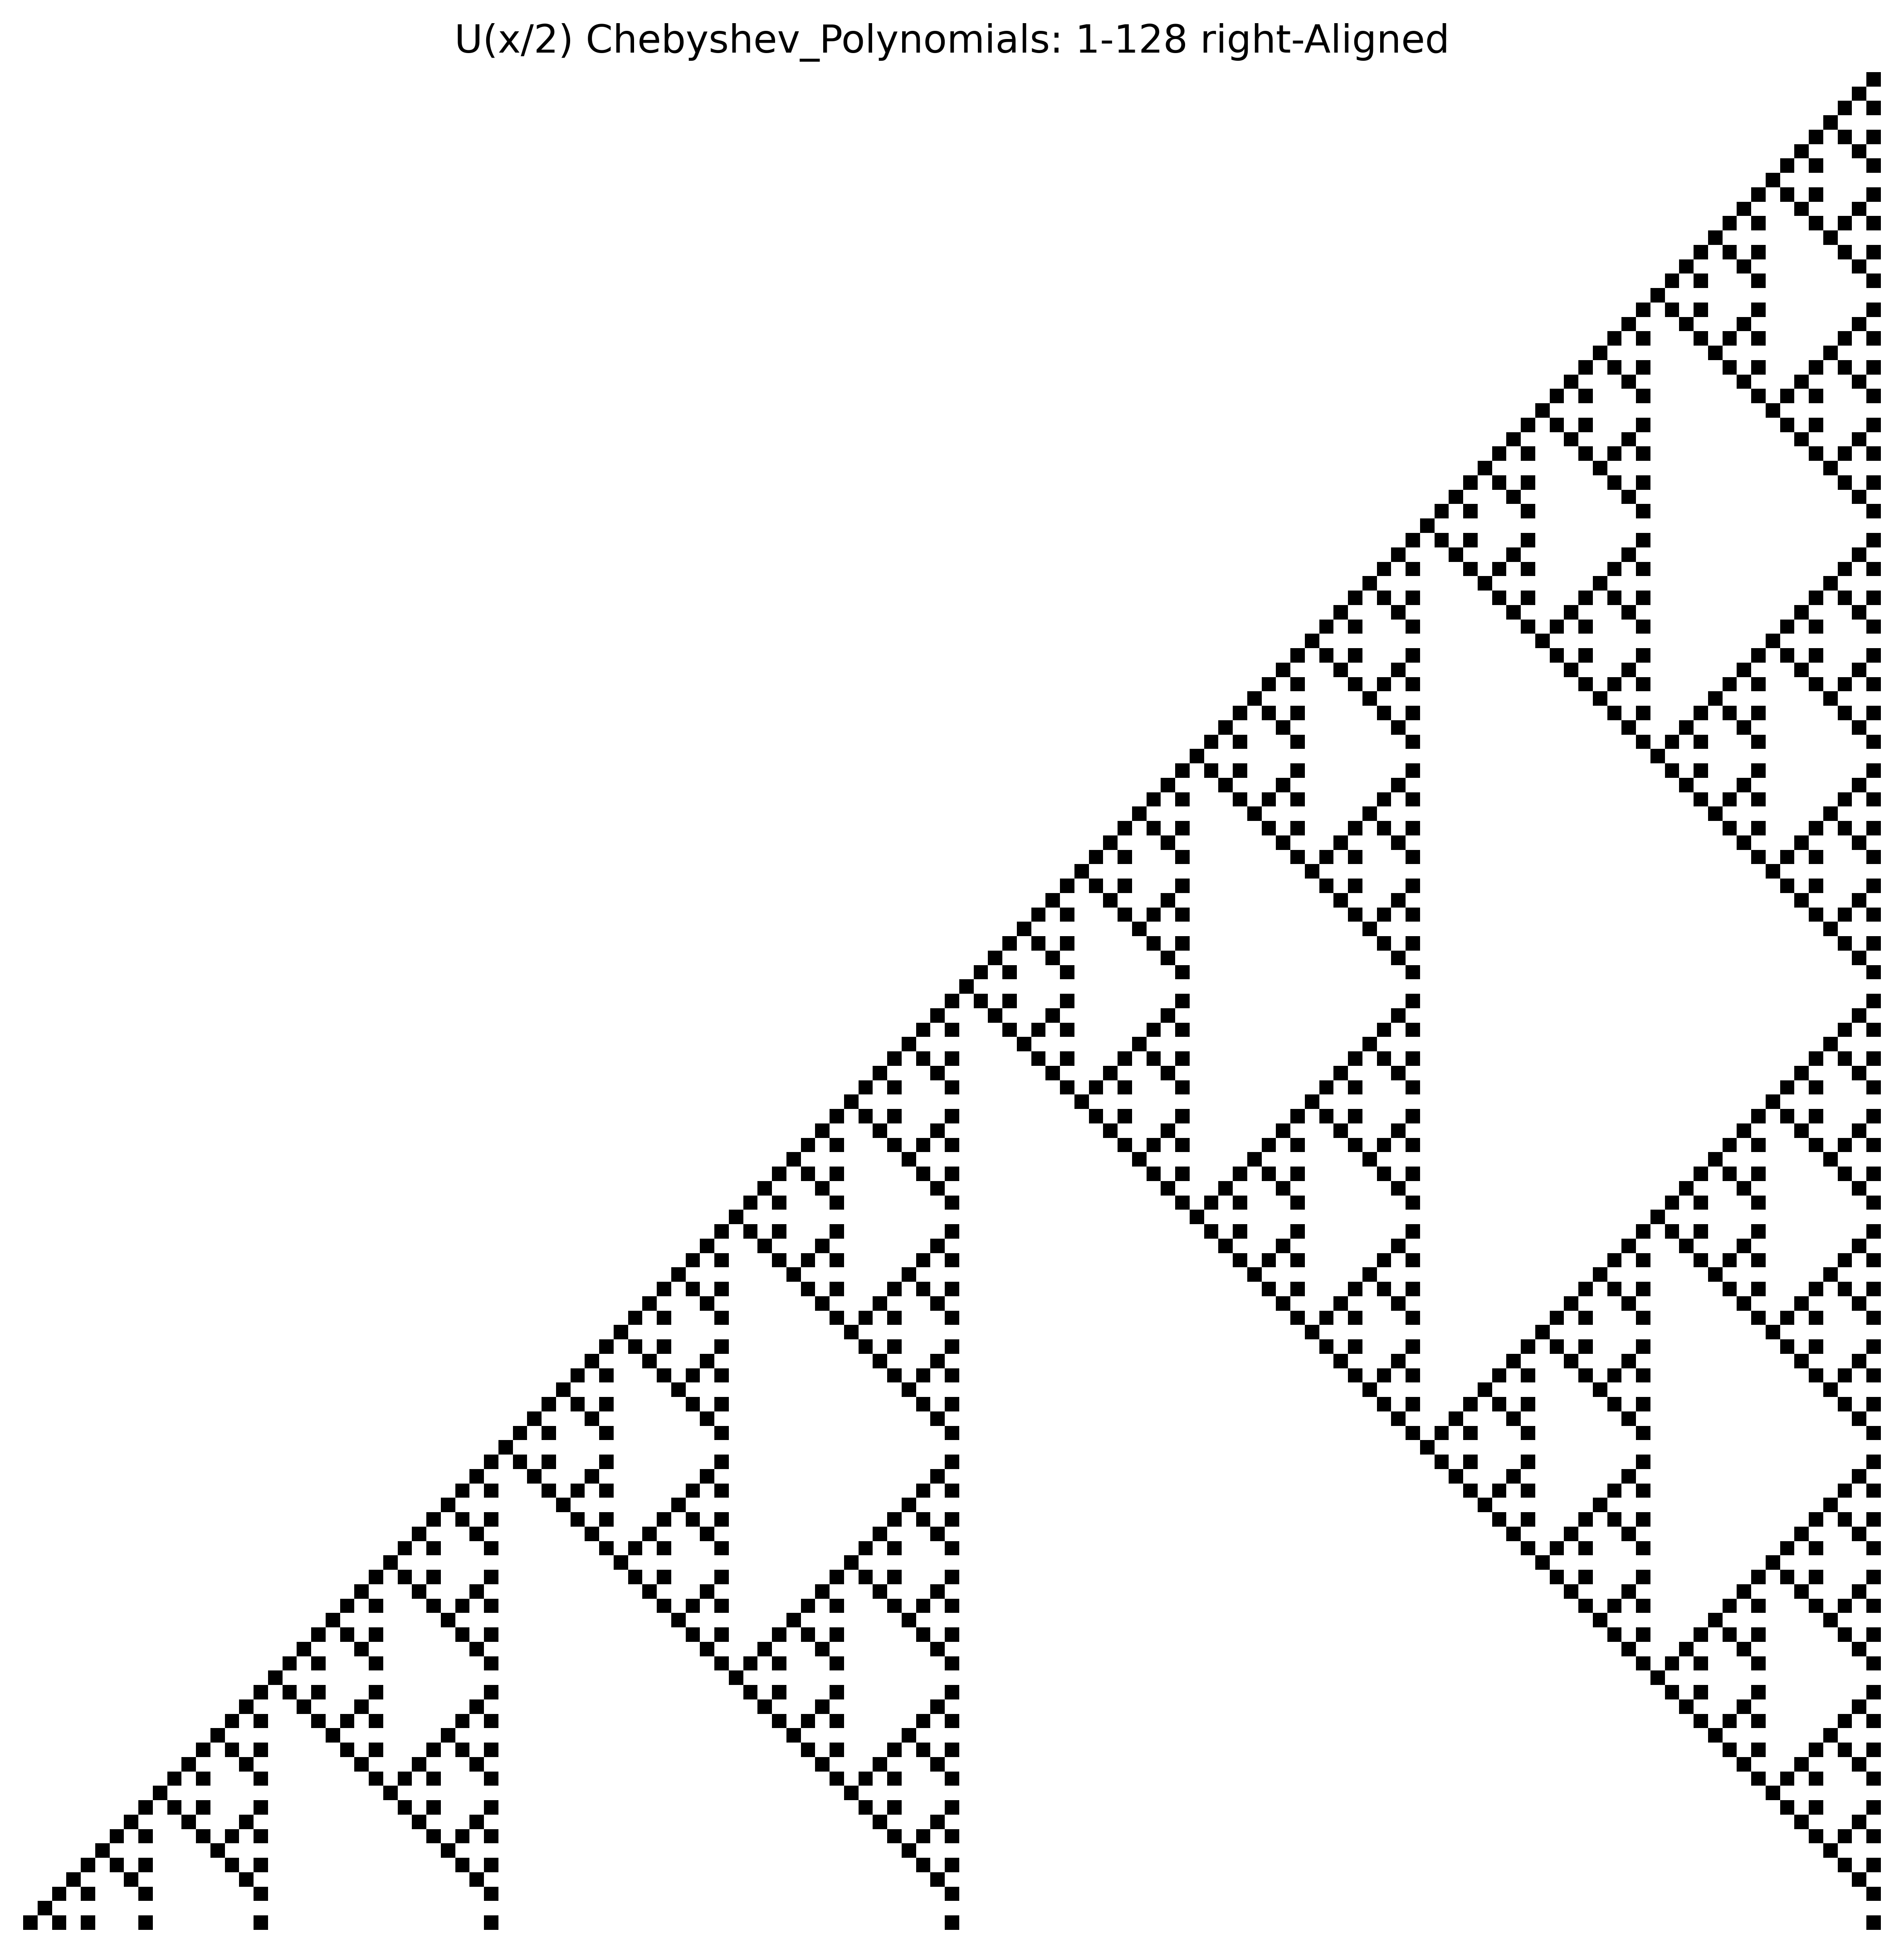
\includegraphics[width=.5\textwidth]{../../code/serialization/chebyshev/chebyshev1_right_128.png}	
	\end{center}

	Those familiar with elementary cellular automata might recognize this as half of rule 90, just rotated on its side.
	\begin{center}
		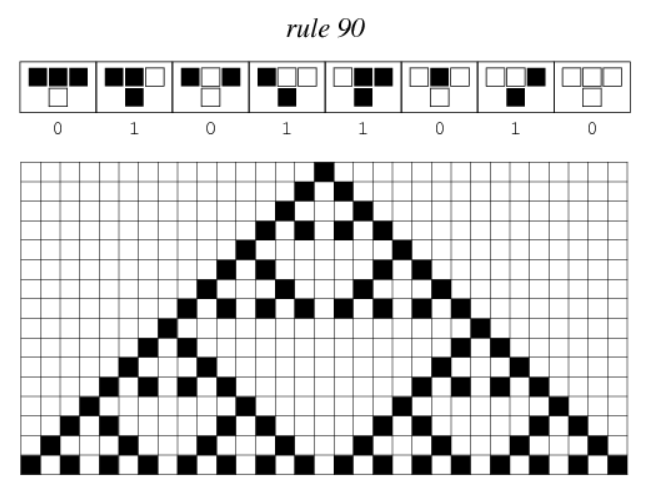
\includegraphics[width=0.5\textwidth]{rule90.png}
	\end{center}

	We'll now show that these are in fact the same pattern, as long as we plot a power of 2 number of terms.
	\begin{lemma}
		For any positive integer $k$, plotting $f(0,x)$ through $f(2^k - 1,x)$ inclusive yields the right half of rule 90. 
	\end{lemma}
	\begin{proof}
		First, note that the first two rows in our image are equal to the last two columns produced by rule 90 after $2^k - 1$ steps.
		So, for $n \leq 2$, our relationships holds.
		
		Assume $n > 2$.
		By the xor definition of $f_n(x)$,
		\begin{equation*}
			f_n(x) = xf_{n-1}(x) \xor f_{n-2}(x).
		\end{equation*}
		Let $f_n(x)_i$ be the $i$th digit in the binary representation of $f_n(x)$, with $i=0$ giving the largest term, and $i=n$ giving the units term.
		For a particular cell,
		\begin{equation*}
			f_n(x)_i = f_{n-1}(x)_i \xor f_{n-2}(x)_{i-2}.
		\end{equation*}
		Rearranging,
		\begin{equation*}
			f_{n-1}(x)_i = f_n(x)_i \xor f_{n-2}(x)_{i-2}.
		\end{equation*}
		This is exactly what rule 90 tells us: The state of a cell in a subsequent row (column in our image) is the XOR of the two cells to the left and right in the above row, and that the cell immediately above does not affect the outcome.
	\end{proof}
	
	\section{Rule 90 \& Binomial Coefficients}
	Now that we know that there is a relationship between our Fibionacci polynomials and rule 90, we'd like a way to calculate these polynomials by determining whether a given cell in rule 90 is on or off.
	One place that rule 90 appears is in Pascal's Triangle of binomial coefficients.
	If each entry in the triangle that is odd is colored black and each entry that is even colored white, then the even rows (0,2,4,...) give exactly rule 90.
	
	\begin{lemma}
		Let $f_n(x)_i$ be the $i$th entry in the coefficient list of $f(n,x)$ so that $f(n,x)_0$ is the highest degree term and $f(n,x)_n$ is the units term.
		Let $K = 2^k - 1$ where $k$ is the smallest integer such that $K \geq n$.
		Let $S = 2(K-n)$.
		Then
		\begin{equation*}
			f(n,x)_i = \binom{2i + S}{S + i} \mod 2.
		\end{equation*}	
	\end{lemma}
	\begin{proof}
		Notice that when working modulo 2,
		\begin{align*}
			\binom{p}{q} &= \binom{p-1}{q} + \binom{p-1}{q-1} \\
				&= \binom{p-2}{q} + \binom{p-2}{q-1} + \binom{p-2}{q-1} + \binom{p-2}{q-2} \\
				&\equiv \binom{p-2}{q} + \binom{p-2}{q-2}.
		\end{align*}
		We see then that the parity of $\binom{p}{q}$ is determined by the parities of $\binom{p-2}{q}$ and $\binom{p-2}{q-2}$ in a XOR fashion.
		That is, for $\binom{p}{q}$ to be odd, the parities of each much by different.
		So, to generate rule 90, we need the parity of even rows in Pascal's Triangle. \\
		
		We saw before that our polynomials plotted out exactly matched rule 90 when we plotted $f_0$ to $f_m$, where $m$ is one less than a power of 2.
		So, $f_n(x)_i$ is found by looking at the $(K-n+i)$th row and $(K-i)$th column in the right half of rule 90, where the 0th row and 0th column is the top and center of rule 90.
		Thus, $f_n(x)_i$ is found by looking at the parity of the $2(K-n+i)$ row and $(K-n)$th column in the right half of Pascal's Triangle.
		That is, the parity of $\binom{2(K-n+i)}{2(K-n) + i} = \binom{S + 2i}{S + i}$.
	\end{proof}

	It turns out that there's a quick way to calculate the parity of binomial coefficients.
	\begin{theorem}[Kummer's Theorem]
		Let $p$ be a prime, $n$ and $m$ positive integers.
		Then the highest power of $p$ that divides $\binom{n+m}{m}$ is the number of carry operations when adding $n$ and $m$ in base $p$.
	\end{theorem}

	Since we just want to know if the binomial coefficient is even, we just to find if there is at least one carry operation when adding in base 2.
	If we are adding two binary numbers that both have a 1 in the same place, then there is a carry operation our of this place.
	The first carry operation that happens must also have two 1 matching in the same place.
	Thus, there is at least one carry operation when adding $n$ and $m$ in binary if and only if $n \texttt{ \& } m \neq 0$, where $\texttt{\&}$ is the bitwise AND operation.
	
	So, we now have an algorithm for calculating $f(n,x)$ in coefficient list form.
	Below is an implementation in Python
	\begin{center}
	\begin{verbatim}
		from math import ceil, log2
			
		def binomial_parity(n: int, m: int) -> int:
    		return 0 if ((n-m) & m) else 1
			
		def f(n: int) -> list[int]:
    		K = (1 << ceil(log2(n + 1))) - 1
    		S = 2*(K - n)
			
    		return [binomial_parity(2*i + S, i + S) for i in range(n+1)]
	\end{verbatim}
	\end{center}

	\section{Identities Relating $f_n(x)$ and $f_{2n+1}(x)$}
	Now that we have an algorithmic way to calculate $f_n(x)$, we can work on deriving some relationships to $f_{2n+1}(x)$.
	
	Define
	\begin{equation*}
		g(b,k) = b 2^{k-1} - 1,
	\end{equation*}
	for any odd natural number $b$ and any natural number $k$.
	
	\begin{lemma}
		For any $n \in \N$, there exists $b$ and $k$ such that
		\begin{equation*}
			n = g(b,k).
		\end{equation*}
	\end{lemma}
	\begin{proof}
		Let $n+1 = 2^{m-1}n'$, where $m \in \N$ and $n' \in \N$ and is odd.
		Then
		\begin{equation*}
			g(n', m) = n'2^{m-1} - 1 = (n+1) - 1 = n,
		\end{equation*}
		as desired.
	\end{proof}
	
	\begin{lemma}
		For all $b$, $k$,
		\begin{equation*}
			g(b,k+1) = 2g(b,k) + 1.
		\end{equation*}
	\end{lemma}
	\begin{proof}
		Notice,
		\begin{align*}
			g(b,k+1) &= b 2^{k} - 1 \\
				&= 2\left(b 2^{k-1} - 1\right) + 1 \\
				&= 2g(b,k) + 1,
		\end{align*}
		as desired.
	\end{proof}
	\begin{lemma}
		Let
		\begin{equation*}
			f_{g(b,k)}(x) = x^{a_1} + x^{a_2} + \dots + x^{a_m}.
		\end{equation*}
		Then
		\begin{equation*}
			f_{g(b,k+1)}(x) = x^{2a_1 + 1} + x^{2a_2 + 1} + \dots + x^{2a_m + 1}.
		\end{equation*}
	\end{lemma}
	\begin{proof}
		Consider how we calculate $f(g(b,k),x)$ in our code.
		\begin{align*}
			K_{g(b,k)} &= 2^{\lceil \log_2{\left(b\cdot2^{k-1}\right)} \rceil} - 1 \\
				&= 2^{\lceil \log_2{\left(2^{k-1}\right)}+ \log_2{(b)} \rceil} - 1 \\
				&= 2^{\lceil k-1 + \log_2{(b)} \rceil} - 1 \\
				&= 2^{k + \lfloor \log_2{(b)} \rfloor} - 1. \\
			S_{g(b,k+1)} &= 2\left(K - \left(b\cdot2^{k-1} - 1\right)\right) \\
				&= 2\left(2^{k + \lfloor \log_2{(b)} \rfloor} - 1 - b\cdot2^{k-1}+1\right) \\
				&= 2\left(2^{k + \lfloor \log_2{(b)} \rfloor} - b\cdot2^{k-1}\right) \\
				&= 2^{k+1+\lfloor\log_2{(b)}\rfloor} - b\cdot2^{k} \\
				&= 2^{k}\left(2^{\lceil \log_2{(b)}\rceil} - b\right).
		\end{align*}
		To calculate to polynomial as a list of coefficients,
		\begin{equation*}
			\left[\binom{S_{g(b,k)} + 2i}{S_{g(b,k)} + i} \mod 2 \texttt{ for i in range(n+1)} \right],
		\end{equation*}
		where
		\begin{equation*}
			\binom{n}{m} \mod 2 = \begin{cases}
				0 & \texttt{((n-m) \& m) != 0} \\
				1 & \text{otherwise}
			\end{cases}.
		\end{equation*}
		For $f_{g(b,k)}(x)$,
		\begin{align*}
			\binom{S_{g(b,k)}+2i}{S_{g(b,k)}+i} \mod 2 &= \binom{2^{k}\left(2^{\lceil \log_2{(b)}\rceil} - b\right) + 2i}{2^{k}\left(2^{\lceil \log_2{(b)}\rceil} - b\right) + i} \mod 2 \\
			&= \begin{cases}
				0 & \texttt{i \& }\left(2^{k}\left(2^{\lceil \log_2{(b)}\rceil} - b\right) \texttt{ + i}\right)\texttt{ != 0} \\
				1 & \text{otherwise}
			\end{cases}.
		\end{align*}
		Imagine that for some $i$, $b$, and $k$ that
		\begin{align*}
			\binom{2^{k}\left(2^{\lceil \log_2{(b)}\rceil} - b\right) + 2i}{2^{k}\left(2^{\lceil \log_2{(b)}\rceil} - b\right) + i} \mod 2 &= 0 \\
			\texttt{i \& }\left(2^{k}\left(2^{\lceil\log_2{(b)}\rceil} - b\right)\texttt{+ i}\right) &\neq 0.
		\end{align*}
		Then
		\begin{align*}
			\texttt{2i \& }2\left(2^{k}\left(2^{\lceil\log_2{(b)}\rceil} - b\right)\texttt{+ i}\right) &\neq 0.
		\end{align*}
		Recall that our list of coefficients represents polynomials with the highest degree as the first term (i.e. index 0).
		Thus, the sum of the index and the degree for $f(n,x)$ is always equal to $n$.
		So, for $f(g(b,k),x)$,
		\begin{align*}
			\deg_{i,k} + i &= g(b,k) \\
			\deg_{i,k} &= g(b,k) - i
		\end{align*}
		where $\deg_{i,k}$ is the corresponding degree of the coefficient at index $i$ in our representation of $f(g(b,k))$.
		So, for $f(g(b,k+1),x)$,
		\begin{align*}
			\deg_{2i,k+1} + 2i &= g(b,k+1) \\
			\deg_{2i,k+1} &= g(b,k+1) - 2i \\
			&= b\cdot2^{k} - 1 - 2i \\
			&= 2\left(b\cdot2^{k-1} - 1 - i\right) + 1 \\
			&= 2\left(g(b,k) - i\right) + 1 \\
			&= 2\deg_{i,k} + 1.
		\end{align*}
		So, we see that
		\begin{equation*}
			\binom{S_{g(b,k)} + 2i}{S_{g(b,k)} + i} \mod 2 = 0 \implies \binom{S_{g(b,k+1)} + 4i}{S_{g(b,k+1)}) + 2i} \mod 2 = 0.
		\end{equation*}
		The same logic applies to show that both sides get the same result if the parity is odd. Thus,
		\begin{equation*}
			\binom{S_{g(b,k)} + 2i}{S_{g(b,k)} + i} \equiv \binom{S_{g(b,k+1)} + 4i}{S_{g(b,k+1)} + 2i} \mod 2.
		\end{equation*}
		Now we just need to consider odd indices $i$ in $f(g(b,k),x)$.
		Recall that for any index $i$,
		\begin{equation*}
			\binom{S_{g(b,k)} + 2i}{S_{g(b,k)} + i} \mod 2 =\begin{cases}
				0 & \texttt{i \& }\left(S_{g(b,k)} + i\right) \neq 0 \\
				1 & \text{otherwise}
			\end{cases}.
		\end{equation*}
		Since $S_{g(b,k)} = 2^k\left(2^{\lceil \log_2{(b)} \rceil} - b\right)$, and $k \in \N$,
		$S_{g(b,k)}$ is always even.
		Thus for odd $i$, both $i$ and $S_{g(b,k)} + i$ will be odd.
		Therefore, the result of their bitwise AND (i.e. \texttt{\&}) will be non-zero.
		So, all odd indices $i$ in $f(g(b,k+1))$ will be 0 in our polynomial representation.
	\end{proof}

	\begin{corollary}
		The following identity holds:
		\begin{equation*}
			f_{2n+1}(x) = x\left(f_{n}(x)\right)^2.
		\end{equation*}
	\end{corollary}
	\begin{proof}
		Let $n = g(b,k)$, so that $2n+1 = g(b,k+1)$.
		Let
		\begin{equation*}
			f_{g(b,k)}(x) = x^{a_1} + x^{a_2} + \dots + x^{a_n},
		\end{equation*}
		where $a_1 > a_2 > \dots > a_n \geq 0$.
		Then
		\begin{align*}
			f_{g(b,k+1)}(x) &= x^{2a_1 + 1} + x^{2a_2 + 1} + \dots + x^{2a_n+1} \\
				&= x\left(x^{2a_1} + x^{2a_2} + \dots + x^{2a_n}\right) \\
				&=\equiv x\left(x^{a_1} + x^{a_2} + \dots + x^{a_n}\right)^2 \\
				&= x\left(f_{g(b,k)}(x)\right)^2 \\
				&= x\left(f_{n}(x)\right)^2,
		\end{align*}
		as desired.
	\end{proof}

	\begin{corollary}
		The following identity holds:
		\begin{equation*}
			f_{2n+1}(x+1) = (x+1)\left(f_{n}(x+1)\right)^2.
		\end{equation*}
	\end{corollary}

	\section{GCDs of Polynomials}
	Now that we have a way to express $f_{2n+1}(x)$ in terms of the product of $f_{n}(x)$ terms and $x$, we simply need a way to express the GCD of products.
	This is where a result from Ore comes in handy \cite{ore_number_theory}
	
	\begin{theorem}[Ore]
		Let $(a,b)$ denote $\gcd{(a,b)}$.
		Then
		\begin{equation*}
			(ab,cd) = (a,c)(b,d)\left(\frac{a}{(a,c)},\frac{d}{(b,d)}\right)\left(\frac{c}{(a,c)},\frac{b}{(b,d)}\right).
		\end{equation*}
	\end{theorem}

	Finally, we are ready to state and prove Sutner's conjecture
	\begin{theorem}
		For all $n \in \N$,
		\begin{equation*}
			d(2n+1) = 2d(n) + \delta_n,
		\end{equation*}
		and $\delta_{2n+1} = \delta_n$.
	\end{theorem}
	\begin{proof}
		Notice,
		\begin{align*}
			d(2n+1) &= \deg \left(f_{2n+1}(x), f_{2n+1}(x+1)\right) \\
				&= \deg \left(xf^2_n(x), (x+1)f^2_n(x+1)\right) \\
				&= \deg (x,x+1)\left(f^2_n(x),f^2_n(x+1)\right)\left(\frac{x+1}{(x,x+1)},\frac{f^2_n(x)}{(f^2_n(x),f^2_n(x+1))}\right)\left(\frac{x}{(x,x+1)},\frac{f^2_n(x+1)}{(f^2_n(x),f^2_n(x+1))}\right) \\
				&= \deg \left(f_n(x),f_n(x+1)\right)^2\left(x+1,\frac{f^2_n(x)}{(f_n(x),f_n(x+1))^2}\right)\left(x,\frac{f^2_n(x+1)}{(f_n(x),f_n(x+1))^2}\right) \\
				&= \deg \left(f_n(x),f_n(x+1)\right)^2\left(x+1,\frac{f_n(x)}{(f_n(x),f_n(x+1))}\right)\left(x,\frac{f_n(x+1)}{(f_n(x),f_n(x+1))}\right) \\
				&= 2d(n) + \deg\left(x+1,\frac{f_n(x)}{(f_n(x),f_n(x+1))}\right)\left(x,\frac{f_n(x+1)}{(f_n(x),f_n(x+1))}\right).
		\end{align*}
		Notice that if we substitute $x+1$ for $x$, 
		\begin{equation*}
			\left(x+1,\frac{f_n(x)}{(f_n(x+1),f_n(x+1+1))}\right) = \left(x+1+1,\frac{f_n(x+1)}{(f_n(x+1+1),f_n(x+1))}\right) = \left(x,\frac{f_n(x+1)}{(f_n(x),f_n(x+1))}\right).
		\end{equation*}
		Thus, we see that these two remaining GCD terms are either both 1 nor not 1 simultaneously.
		This means we can further simplify to
		\begin{equation*}
			d(2n+1) = 2d(n) + 2\deg\left(x,\frac{f_n(x+1)}{(f_n(x),f_n(x+1))}\right).
		\end{equation*}
		So, we see that
		\begin{equation*}
			d(2n+1) = 2d(n) + \delta_n \text{, where }\delta_n = 2\deg\left(x,\frac{f_n(x+1)}{(f_n(x),f_n(x+1))}\right) = 2\deg\left(x+1,\frac{f_n(x)}{(f_n(x),f_n(x+1))}\right).
		\end{equation*}
		Thus, $\delta_n \in \{0,2\}$. \\
		
		Next, we'll calculate $\delta_{2n+1}$.
		First, notice that
		\begin{equation*}
			f_{2(2n+1)+1}(x) = xf^2_{2n+1}(x) = x\left(xf^2_n(x)\right)^2 = x^3f^4_n(x).
		\end{equation*}
		So,
		\begin{align*}
			d(2(2n+1)+1) &= \deg\left(x^3f^4_n(x), (x+1)^3f^4_n(x+1)\right) \\
				&= \deg\left(x,(x+1)^3\right)\left(f^4_n(x),f^4_n(x+1)\right)\left(x^3,\frac{f^4_n(x+1)}{(f^4_n(x),f^4_n(x+1))}\right)\left((x+1)^3,\frac{f^4_n(x)}{(f^4_n(x),f^4_n(x+1))}\right) \\
				&= \deg\left(f_n(x),f_n(x+1)\right)^4\left(x^3,\frac{f^4_n(x+1)}{(f_n(x),f_n(x+1))^4}\right)\left((x+1)^3,\frac{f^4_n(x)}{(f_n(x),f_n(x+1))^4}\right) \\
				&= \deg\left(f_n(x),f_n(x+1)\right)^4\left(x^3,\frac{f^3_n(x+1)}{(f_n(x),f_n(x+1))^3}\right)\left((x+1)^3,\frac{f^3_n(x)}{(f_n(x),f_n(x+1))^3}\right) \\
				&= \deg\left(f_n(x),f_n(x+1)\right)^4\left(x,\frac{f_n(x+1)}{(f_n(x),f_n(x+1))}\right)^3\left((x+1),\frac{f_n(x)}{(f_n(x),f_n(x+1))}\right)^3 \\
				&= 4d(n) + 3\delta_n.
		\end{align*}
		Also,
		\begin{align*}
			d(2(2n+1)+1) &= 2d(2n+1) + \delta_{2n+1} \\
				&= 2\left(2d(n) + \delta_n\right) + \delta_{2n+1} \\
				&= 4d(n) + 2\delta_n + \delta_{2n+1}.
		\end{align*}
		For these two expressions for $d(2(2n+1)+1)$ to be equal, we must have $\delta_{2n+1} = \delta_n$.
	\end{proof}
	
	\newpage
	\bibliography{refs.bib}
	\bibliographystyle{amsplain}
\end{document}